\section{Using Matrix Factorization for Imputation}  \label{sec:mf}

% need update and to be consistent with related work, need to add the Netflix and our KDD2011 papers to support MF

Matrix Factorization (MF) is arguably the most successful Collaborative Filtering~(CF) technique in the area of Recommendation Systems~\cite{koren2009matrix, chen2011linear}. Comparing to other recommendation models such as regression-based prediction models, graph-based random walk models, or simple statistical models, the MF model possesses the advantages of being more accurate and more scalable to data size.
A key feature of MF models is its capability to learn latent factors from relatively sparse observations, and to leverage these factors to impute the missing elements in the matrix.
In the following, we will first introduce the fundamentals of the MF methodology, present our novel sensor-data-specific 
modifications to the MF objective function, and finally provide the complete training procedure of the proposed method.

\subsection{Introducing Matrix Factorization}

%, a widely known dimension reduction technique, 
%in dealing with incomplete or sparse data.
%The goal of SVD is to decompose a fully observed matrix~$\mathbf{R}$ into one diagonal matrix~$\mathbf{D}$ and two unitary matrices~$\mathbf{U}$ and~$\mathbf{V}$ such that
%%\begin{equation*} 
%$\mathbf{R} = \mathbf{U}\mathbf{D}\mathbf{V}^T.$ %\end{equation*}
%The largest $K$ singular values and vectors, $\mathbf{U}_K \mathbf{D}_K \mathbf{V}_K^T$, form the best $K$-rank approximation of $\mathbf{R}$ under the Frobenius Norm. Unfortunately, conventional SVD cannot be performed when the matrix~$\mathbf{R}$ is incomplete. 
%Therefore, to exploit latent dimensions through SVD for imputation, prior work (such as EOF) has to fill in missing entries first 
%(usually using zeros or an averaged value) and then perform dimension reduction through retaining the largest $K$ singular values~\cite{beckers2003eof}. 
%Such strategy does create some dilemmas as a high-quality imputation model is needed in the first stage to guarantee the quality of 
%data reproduced in the later stage, but it is such high-quality that we seek for data imputation. In a nutshell, SVD, although 
%proven to be ideal for dimension reduction, can hardly be applied to sparse matrices where a significant fraction of 
%the data are missing.
%
As stated in section \ref{sec:existing_work}, conventional SVD is not appropriate for the task of missing data imputation.
Matrix Factorization is designed to amend the limitations of SVD, and recently researchers have shown \cite{koren2009matrix} that the matrix factorization model is indeed a better approach to learn the latent factors given sparse matrices, because during the factorization procedure only the observed entries are exploited.
Utilizing numerical optimization procedures, for a partially observed matrix~$\mathbf{R}$, MF produces two latent 
matrices~$\mathbf{P}_{M \times K}$ and $\mathbf{Q}_{K \times N}$ whose multiplication seeks to approximate the observed entries in $\mathbf{R}_{M \times N}$:
\begin{equation*}\small \mathbf{R} \approx \mathbf{P} \mathbf{Q}.\end{equation*}
Given $\mathbf{R}$ being the sensor network readings, each row of $\mathbf{P}$ represents latent factors in the temporal dimension and each column of $\mathbf{Q}$ represents the latent factors in the dimension of correlation among sensors.

We adopt the biased-MF which includes row and column biases $\mu_m$ and $\mu_n$. 
In a temperature monitoring system, the row bias can be understood as the average temperature at a given time, and the column bias reflects the average temperature at the location plus the systematic bias of the sensor node.
The predictions of missing values can be obtained through $\hat{r}_{mn} = \mu_m + \mu_n + \mathbf{p}_m \mathbf{q}_n$.
After adding the regularization term to constraint the scale of latent factors, the objective function of MF becomes to minimize:
\begin{equation*}\small \begin{aligned}
\frac{1}{2}\sum_{m,n}{(r_{mn} - \hat{r}_{mn})}^2
+ \frac{\beta}{2}(\sum_m{(\mu_m^2 + ||\mathbf{p}_m||^2)} + \sum_n{(\mu_n^2 + ||\mathbf{q}_n||^2)}),
\end{aligned}\end{equation*}
where $\mathbf{p}_m$ are the row factors of $\mathbf{P}$ (for time $m$), and $\mathbf{q}_n$ are the column factors of $\mathbf{Q}$ (for sensor node $n$) respectively.
$\beta$ is the parameter that controls the strength of regularization.

\subsection{Temporally-Regularized Matrix Factorization}
\begin{figure}[htbp]
	\centering
	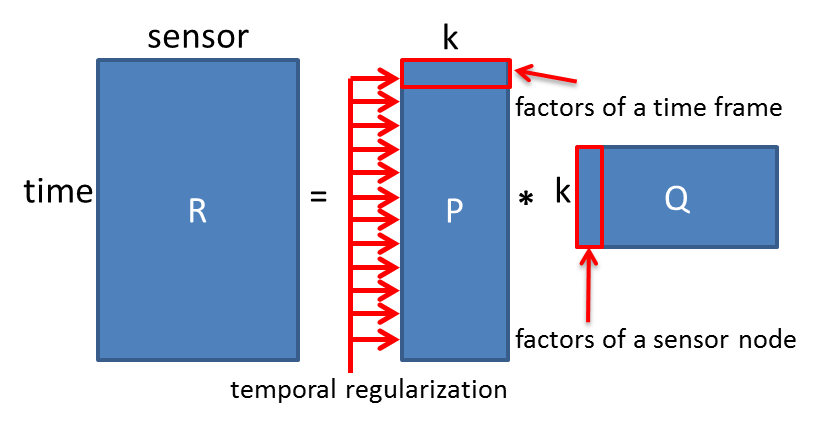
\includegraphics[width=0.4\textwidth]{TRMF_illustration.png}
	\caption{illustration of TR-MF}
\end{figure}
%cite temporal reference
Although we map the sensor data imputation task to a CF-based recommendation task, there are indeed some major differences in terms of the property of data.
Normal CF or MF models assume the users (i.e., temporal dimension) are independent of each other. That is, we can randomly swap the columns in the matrix without affected the factorization outcome. However, such independence does not exist in sensor data as a 
sensor's signal in time $t$ is highly dependent on that of time $t-1$. In other words, an ideal model should consider such order dependency, and under such a model the swap of columns shall significantly affect the outcome of factorization.

With this observation, we propose a Temporally-Regularized Matrix Factorization (TR-MF) to better model the characteristic of sensor data. As the name may suggest, TR-MF adds a temporal regularization term to conventional MF.
The temporal regularization forces the latent factors of adjacent rows to be similar, which reflects the fact that 
readings in adjacent time steps should be similar. We also add similar regularization term for row bias.
The modified objective function looks like: 
\begin{equation*}\small \begin{aligned}
\frac{1}{2}\sum_{m,n}{(r_{mn} - \hat{r}_{mn})}^2
&+ \frac{\beta}{2}(\sum_m{(\mu_m^2 + ||\mathbf{p}_m||^2)} + \sum_n{(\mu_n^2 + ||\mathbf{q}_n||^2)}) \\
&+ \frac{\gamma}{2} \sum{((\mu_m-\mu_{m+1})^2 + ||\mathbf{p}_m-\mathbf{p}_{m+1}||^2)}.
\end{aligned}\end{equation*}

\subsection{Spatio-Temporal-Regularized Matrix Factorization}
%A strong argument that directly exploiting spatial information to specify the assumed inter-sensor node correlation may not be as good as directly learning these correlations directly from the sensor observations themselves.
Although previously we argue that nearby sensors might not necessarily possess the highest correlation with each other, 
here we would like to show that our TR-MF model can easily be extended to accommodate spatial correlation if one decides to do so. 
Given the distance (or any kind of `closeness' measure) between sensors, we can add spatial regularization terms to bias for 
possible spatial correlation.
The objective function then becomes: 
\begin{equation*}\small \begin{aligned}
\frac{1}{2}\sum_{m,n}{(r_{mn} - \hat{r}_{mn})}^2
&+ \frac{\beta}{2}(\sum_m{(\mu_m^2 + ||\mathbf{p}_m||^2)} + \sum_n{(\mu_n^2 + ||\mathbf{q}_n||^2)}) \\
&+ \frac{\gamma_1}{2} \sum{((\mu_m-\mu_{m+1})^2 + ||\mathbf{p}_m-\mathbf{p}_{m+1}||^2)}\\
&+ \frac{\gamma_2}{2} \sum{((\mu_{n_i}-\mu_{n_j})^2 + ||\mathbf{p}_{n_i}-\mathbf{p}_{n_j}||^2)}.
\end{aligned}\end{equation*}
We call this Spatio-Temporal-Regularized Matrix Factorization (STR-MF). Note that we suggest users to exploit spatial 
regularization with care, as our experimental study will show that biasing for spacial correlation can often produce inferior results. 
In the following discussion, we will mainly focus on TR-MF.

\subsection{Optimization Procedure}
\label{optimation_procedure}
Several methods to learn MF have been proposed, such as Stochastic Gradient Descent (SGD)\cite{koren2009matrix,chih2008large}, Alternating Least Square (ALS)\cite{koren2009matrix,zhou2008large}, Newton's method\cite{buchanan2005damped} and Wiberg Algorithm\cite{okatani2007wiberg}.
For sensor data, we suggest SGD for its efficiency and simplicity. 

In SGD, we incrementally update our model by considering one reading at a time.
Focused on one observed reading $r_{mn}$ with the following objective function
\begin{equation*} \small \frac{1}{2}(r_{mn} - \hat{r}_{mn})^2
+ \frac{\beta}{2}(\mu_m^2 + \mu_n^2 + ||\mathbf{p}_m||^2 + ||\mathbf{q}_n||^2).\end{equation*}
It is not hard to derive the update equations as \\
\indent	$ \begin{cases} 
	\mu_m' = \mu_m - \eta ((\hat{r}_{mn}-r_{mn}) + \beta \mu_m) \\
	\mu_n' = \mu_n - \eta ((\hat{r}_{mn}-r_{mn}) + \beta \mu_n) \\
	\mathbf{p}_{m}' = \mathbf{p}_{m} - \eta ((\hat{r}_{mn}-r_{mn})\mathbf{q}_{n} + \beta \mathbf{p}_{m})\\
	\mathbf{q}_{n}' = \mathbf{q}_{n} - \eta ((\hat{r}_{mn}-r_{mn})\mathbf{p}_{m} + \beta \mathbf{q}_{n})\\
	\end{cases} $ \\
For each reading, we update all the $\mu_m$ and $\mathbf{p}_m$. Then after a full scan of all observed readings, 
we perform temporal regularization by updating all $\mu_m$ and $\mathbf{p}_m$ simultaneously according to the following equations:\\
\indent $ \begin{cases}
	\mu_m' = \mu_m - \eta \gamma_1((\mu_m-\mu_{m-1})+(\mu_m-\mu_{m+1}))\\
	\mathbf{p}_{m}' = \mathbf{p}_{m} - \eta \gamma_1((\mathbf{p}_{m}-\mathbf{p}_{m-1})+(\mathbf{p}_{m}-\mathbf{p}_{m+1}))\\
	\end{cases} $\\
The updating procedure is summarized in Procedure~\ref{alg:STRMF}. Note that we propose to avoid updating the temporal regularization with the update of each reading, because doing so can bias the model toward the time steps that possess fewer missing readings, which contradicts the goal of data imputation. 

If the spatial regularization is exploited, we can update all $\mu_n$ and $\mathbf{q_n}$ simultaneously as:\\
\indent $\begin{cases}
	\mu_{n_i}' = \mu_{n_i} - \eta \gamma_2 \sum_{n_j}{(\mu_{n_i} - \mu_{n_j})}\\
	\mathbf{q_{n_i}}' = \mathbf{q_{n_i}} - \eta \gamma_2 \sum_{n_j}{(\mathbf{q_{n_i}} - \mathbf{q_{n_j}})}\\
	\end{cases}$\\
where $n_i$ and $n_j$ is a pair of neighboring sensor nodes.

\paragraph*{Data Normalization}
Unlike the ratings in recommendation systems that are normally within certain range (e.g., 1 star to 5 star), readings from WSNs are real-valued (rounded to a desired level of precision), and the range may vary with the sensors.
Here we propose to normalize the training set to zero mean and unit variance before conducting MF learning, and once the missing values are produced by our model, we need to rescale the values to the original mean and variance.
Although this procedure does not change the quality of outcomes theoretically, in practice we do find some benefits: 
First, when the global mean becomes zero, the origin of our model naturally becomes a fine initial point for MF training, which is very important for non-convex optimization techniques such as MF.
Second, normalization forces different datasets to look similar, which simplifies the parameter tuning task. 


%\paragraph*{Parameters Setting}
%There are several parameters in our model: conventional regularization for user biases~$\beta_1$, item biases~$\beta_2$, user factors~$\beta_3$, item factors~$\beta_4$, temporal regularization for biases~$\gamma_1$ and for factors~$\gamma_2$, spatial regularization for biases~$\gamma_3$ and for factors$~\gamma_4$, learning rate for biases~$\eta_1$ and for factors~$\eta_2$, number of factors~$K$, and it can be time consuming to search for a good combination. 
%Here we provide some empirical suggestions to reduce the search space while still obtaining results with decent quality: the rule of thumb is to setup parameters of similar physical meanings to be identical. For example: the following setup is what we exploited for the experiments:
%$ \beta_1 = \beta_2 = \beta_3 = \beta_4, \gamma_1 = \gamma_2, \gamma_3 = \gamma_4, \eta_1 = \eta_2$. %\end{equation*}
%Advanced discussion on this aspect appears later in Section~\ref{subsec:parameter}.
%The parameters in our model are conventional regularization~$\beta$, temporal regularization~$\gamma$, learning rate~$\eta$, number of factors~$K$.
%A too small~$\eta$ or a too large~$K$ can slow down the training process, but it won't degrade the model.
\paragraph*{Stopping Criterion}
The validation set is used to determine the parameters and when to cease updating the MF model. More specifically, the training stops when the validation error keeps increasing for a certain amount of iterations (currently setup to $500$). 

\begin{algorithm}
	\caption{(Spatio-)Temporally-Regularized MF}
	\label{alg:STRMF}
	\textbf{Parameters:} $\beta$, $\gamma$, $\eta$, $K$\\
	\textbf{Input:} training set, validation set
	\begin{algorithmic}
		\State Normalize the training set as $\mathcal{D}$
		\State Initialize $\mu_m$, $\mu_n$, $\mathbf{p}_m$, $\mathbf{q}_n$ to small random numbers
		\Repeat
			\State \textbf{for} each observed reading $r_{mn}$ in $\mathcal{D}$
				\State \indent Update $\mu_m$, $\mu_n$, $\mathbf{p}_{m}$, $\mathbf{q}_{n}$
			\State Update $\mu_m$, $\mathbf{p}_m$ by temporal regularization
			\State (Update $\mu_n$, $\mathbf{q}_n$ by spatial regularization)
		\Until{stopping criterion is met}
		\State Output the model for testing set prediction
	\end{algorithmic}
\end{algorithm}
